\chapter{Cifras de Bloco}
\label{cha:cifras-de-bloco}

No capítulo anterior, vimos que é possível construir um sistema criptográfico seguro contra ataques do tipo ``ciphertext only'' (onde o atacante só tem acesso ao texto cifrado).
Para que isso seja viável, é necessário supor a existência de um gerador de números pseudo-aleatórios, ou seja, um algoritmo capaz de gerar uma sequência de bits que, para todos os efeitos práticos, não pode ser distinguida de uma sequência realmente aleatória.

Embora essa definição de segurança seja um pouco mais fraca do que a apresentada no Capítulo \ref{cha:sigilo-perfeito}, ela tem a vantagem de não exigir chaves extremamente longas.
No entanto, assim como o ``One-Time Pad'' (OTP), as cifras de fluxo também apresentam dois problemas importantes:
se uma chave for reutilizada, a segurança é completamente comprometida, e se o adversário souber partes da mensagem original, não há garantias de segurança.

O modelo das cifras de fluxo é ideal para descrever as Máquinas Enigma, utilizadas pelo exército nazista durante a década de 1940.
A cifra empregada por essas máquinas foi quebrada não apenas pelo avanço tecnológico, que possibilitou a construção da máquina Bombe e do computador Colossus, mas também porque os aliados conseguiram obter trechos de mensagens já descriptografadas.

Com base na teoria da criptografia moderna, podemos afirmar que o tipo de ataque realizado pelos ingleses é classificado como um ataque de ``known plaintext'', onde o atacante tem acesso tanto ao texto cifrado quanto a uma versão conhecida do texto original.

Neste capítulo, vamos explorar um modelo de ataque ainda mais poderoso: os ataques do tipo chosen plaintext (CPA). Nesses ataques, o adversário não apenas tem acesso ao texto cifrado, mas também pode escolher mensagens específicas e observar como o sistema as cifra \cite{Bellare97}.

É importante notar que os ataques known plaintext são um caso particular desse modelo mais geral, mas há situações em que devemos considerar que o adversário possui essa capacidade adicional, o que torna o cenário de segurança ainda mais desafiador.


Vamos explicar a segurança contra ataques do tipo \textit{chosen plaintext} (CPA) de maneira semelhante à segurança contra ataques em que o adversário só tem acesso ao texto cifrado (\textit{ciphertext only}). A garantia de segurança que buscamos continua sendo a mesma que discutimos anteriormente, mas agora vamos considerar um cenário de ameaças mais poderoso.

O modelo pode ser descrito da seguinte forma:

\begin{enumerate}
    \item O adversário, $\mathcal{A}$, escolhe duas mensagens de mesmo tamanho, $m_0$ e $m_1$, e as envia para o sistema de criptografia $\Pi$.
    \item O sistema gera uma chave secreta e escolhe aleatoriamente uma dessas mensagens para criptografar.
    \item Durante o processo, e mesmo depois de receber o texto cifrado, o adversário pode perguntar ao sistema como outras mensagens escolhidas por ele seriam cifradas.
    \item O sistema então retorna o texto cifrado para o adversário.
    \item Com base nas informações disponíveis, o adversário tenta adivinhar qual das duas mensagens foi cifrada.
\end{enumerate}

\begin{center}
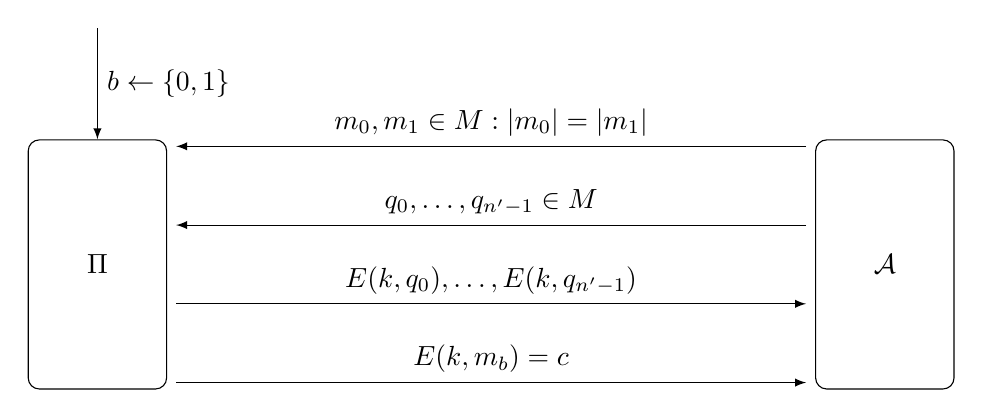
\begin{tikzpicture}[node distance=2cm,auto,>=latex]
\tikzset{
  player/.style={draw,shape=rectangle,rounded corners,minimum width=5em,minimum height=9em}
}
\node[player] (system) {$\Pi$};
\node[player] (adversary) at (10,0) {$\mathcal{A}$};
\draw[->] (9,1.5) -> node[above]{$m_0, m_1 \in M : |m_0| = |m_1|$} (1,1.5);
\draw[->] (9,0.5) -> node[above]{$q_0, \dots, q_{n'-1} \in M$} (1,0.5);
\draw[->] (1,-0.5) -> node[above]{$E(k, q_0), \dots, E(k, q_{n'-1})$} (9,-0.5);
\draw[->] (1,-1.5) -> node[above]{$E(k,m_b) = c$} (9,-1.5);
\draw[->] (0,3) -> node{$b \leftarrow \{0,1\}$} (system);
\end{tikzpicture}
\end{center}

Um sistema é {\em seguro contra CPA} se nenhum adversário polinomial tiver uma vantagem significativa para vencer o jogo que acabamos de descrever.
Ou seja, a probabilidade de que um adversário consiga vencer o jogo é apenas desprezivelmente maior do que $\frac{1}/{2}$

Para construir um sistema seguro contra ataques CPA, precisamos usar o conceito de funções pseudoaleatórias.
Em termos simples, uma função pseudoaleatória é um processo que transforma uma entrada (um conjunto de bits) em uma saída que parece aleatória.

A diferença principal é que a função pseudoaleatória não apenas estende ou gera uma sequência longa a partir de um pequeno pedaço de informação (como um gerador de números pseudoaleatórios faria), mas sim utiliza uma chave para definir a própria função que realiza essa transformação.
Em outras palavras, a chave é usada para escolher a função específica dentro de um grande conjunto de funções possíveis.
Quando aplicamos essa função a uma entrada, ela ``embaralha'' os bits de maneira que a saída pareça aleatória, mesmo sendo gerada de forma determinística.

A segurança de uma função pseudoaleatória é garantida pelo fato de que não existe um algoritmo eficiente (ou seja, que funcione em tempo polinomial) capaz de distinguir entre uma função pseudoaleatória e uma função escolhida de maneira verdadeiramente aleatória.
Em outras palavras, para qualquer adversário que tente diferenciar entre essas duas situações, a função pseudoaleatória será tão boa quanto uma função completamente aleatória.

Uma {\em cifra de bloco} é um tipo específico de função pseudoaleatória, que chamamos de {\em permutação pseudoaleatória}.
Sua característica distintiva é a capacidade de reverter o processo de ``embaralhamento'' dos bits.
Isso significa que, além de transformar uma mensagem de tamanho fixo (o {\em bloco}) em uma saída que parece aleatória, ela também permite que essa transformação seja desfeita de forma eficiente, recuperando a mensagem original.

Assim como outras funções pseudoaleatórias, a cifra de bloco utiliza uma chave para definir como os bits serão embaralhados.
A segurança dessa cifra vem do fato de que, para um adversário, ela é indistinguível de uma permutação completamente aleatória.
Ou seja, não existe um método eficiente para diferenciar entre o comportamento da cifra de bloco e o de uma função que simplesmente embaralha os bits de maneira aleatória.

Na próxima seção, veremos como essas cifras de bloco podem ser combinadas para criptografar mensagens de qualquer tamanho, mantendo a segurança do sistema criptográfico.

\section{Modos de Operação}
\label{sec:modos-de-operacao-bloco}

Uma cifra de bloco é usada para criptografar informações em pedaços de tamanho fixo, chamados de blocos.
No entanto, na prática, muitas vezes precisamos criptografar mensagens que são maiores ou menores que esse tamanho fixo.
Para lidar com isso, precisamos de uma forma de combinar os blocos criptografados pela cifra de bloco para proteger a mensagem inteira.

Uma maneira simples e intuitiva de fazer isso é chamada de {\em Electronic Code Book} (ECB).
Nesse modo de operação, dividimos a mensagem em vários blocos do mesmo tamanho e, em seguida, criptografamos cada um desses blocos separadamente com a cifra de bloco.
Depois de criptografar todos os blocos, simplesmente juntamos os blocos cifrados para formar a mensagem final cifrada.

No entanto, esse método tem uma grande falha de segurança:
blocos idênticos na mensagem original serão criptografados da mesma maneira, resultando em blocos idênticos no texto cifrado.
Isso significa que, se um adversário observar blocos repetidos no texto cifrado, ele pode deduzir que partes da mensagem original são iguais, o que compromete a segurança.

Por exemplo, imagine que um adversário queira descobrir se duas partes de uma mensagem criptografada são iguais ou diferentes.
Ele pode criar duas mensagens de teste:
uma onde a mesma parte se repete, e outra onde as duas partes são diferentes.

Se ele criptografar essas mensagens e o texto cifrado resultar em dois blocos idênticos, o adversário saberá que a mensagem original tinha partes iguais.
Se os blocos cifrados forem diferentes, ele saberá que as partes da mensagem original também eram diferentes.

Em outras palavras, esse adversário consegue distinguir entre as duas cifras ao observar como cada bloco é criptografado.
Isso significa que o modo ECB não é seguro nem mesmo contra ataques apenas contra a cifra.
A Figura \ref{fig:ecb-exemplo} ilustra essa vulnerabilidade.\footnote{Imagem tirada do verbete {\em Modo de Operação (criptografia)} da Wikipédia (\url{https://pt.wikipedia.org})}).

\begin{figure}[!htp]
  \label{fig:ecb-exemplo}
  \centering
  \includegraphics[width=.3\textwidth]{imagens/Tux.jpg}
  \includegraphics[width=.3\textwidth]{imagens/Tux_ecb.jpg}
  \caption{Imagem criptografada no modo ECB}
\end{figure}

Essa forma ingênua de combinar os blocos não garante a segurança contra os tipos de ataques mais básicos que discutimos anteriormente.
O que realmente precisamos é de um sistema que seja seguro contra ataques CPA, onde o adversário pode escolher mensagens e ver como elas são criptografadas.

Na definição de segurança contra CPA, o adversário tem a capacidade de ``consultar'' o sistema para descobrir como uma mensagem específica seria criptografada.
Isso significa que, para proteger o sistema, o processo de criptografia precisa ser imprevisível, ou seja, não pode produzir o mesmo resultado toda vez que a mesma mensagem é criptografada.
Se fosse previsível, o adversário poderia facilmente enganar o sistema ao enviar mensagens que ele já consultou antes.

Para garantir essa imprevisibilidade, incluímos um bloco aleatório no início de cada mensagem, conhecido como {\em vetor inicial} (IV).
Esse vetor inicial não precisa ser mantido em segredo, mas ele assegura que cada vez que uma mensagem é criptografada, o resultado será diferente, mesmo que a mensagem original seja a mesma.
Assim como nas cifras de fluxo, o vetor inicial é fundamental para evitar que padrões previsíveis apareçam no texto cifrado, aumentando a segurança do sistema.

No modo de operação {\em Encadeamento de Blocos de Cifra} ou {\em Cipher Block Chaining} (CBC), cada bloco de texto cifrado não depende apenas da cifra de bloco aplicada ao bloco de texto original, mas também do bloco cifrado que veio imediatamente antes dele.
Isso cria uma ``cadeia'' onde cada bloco cifrado influencia o próximo, aumentando a segurança do processo.

O funcionamento é o seguinte:

\begin{itemize}
\item Primeiro, temos um bloco aleatório inicial, o vetor inicial (IV), que inicia o processo ($c_0 = IV$).
  Esse bloco serve para garantir que cada mensagem cifrada será única.
\item Em seguida, cada bloco da mensagem original é combinado com o bloco cifrado anterior antes de ser criptografado ($p_k(c_{i-1} \xor m_i)$).
  Isso significa que, para criptografar um bloco da mensagem, usamos a cifra de bloco, mas também consideramos o resultado do bloco anterior.
\end{itemize}

Essa cadeia de dependência faz com que, mesmo que dois blocos da mensagem original sejam iguais, seus blocos cifrados finais sejam diferentes, porque cada um deles leva em conta o bloco anterior.
Ao final, o resultado é uma sequência de blocos cifrados, onde cada um depende do anterior, tornando o sistema muito mais seguro.

\begin{center}
\begin{tikzpicture}[node distance=2cm,auto,>=latex]
  \node (IVm) at (0,0)  {$IV$};
  \node (IVc) at (0,-3)  {$IV$};
  \node (m1) at (2,0)  {$m_1$};
  \node (xor1) at (2,-1)  {$\xor$};
  \node (c1) at (2,-3)  {$c_1$};
  \node (m2) at (4,0) {$m_2$};
  \node (xor2) at (4,-1)  {$\xor$};
  \node (c2) at (4,-3) {$c_2$};
  \node at (6,0) {\dots};
  \node at (6,-3) {\dots};
  \node (ml) at (8,0) {$m_l$};
  \node (xorl) at (8,-1)  {$\xor$};
  \node (cl) at (8,-3) {$c_l$};
  \draw[->] (IVm) -> (IVc);
  \draw[->] (IVc) -> (xor1);
  \draw[->] (m1) -> (xor1);
  \draw[->] (xor1) -> node[right]{$p_k$} (c1);
  \draw[->] (c1) -> (xor2);
  \draw[->] (m2) -> (xor2);
  \draw[->] (xor2) -> node[right]{$p_k$} (c2);
  \draw[->] (7,-1) -> (xorl);
  \draw[->] (ml) -> (xorl);
  \draw[->] (xorl) -> node[right]{$p_k$} (cl);
\end{tikzpicture}
\end{center}

Para descriptografar uma mensagem que foi cifrada usando o modo CBC, o processo é basicamente o inverso da criptografia.

Cada bloco da mensagem original é recuperado usando o bloco cifrado correspondente e o bloco cifrado anterior.
Em outras palavras, para descriptografar um bloco específico, aplicamos o processo inverso da cifra de bloco ao bloco cifrado seguinte e, em seguida, combinamos esse resultado com o bloco cifrado anterior ($m_{i}  :=  p_k^{-1}(c_{i+1}) \xor c_{i}$).

Esse processo continua ao longo de toda a sequência de blocos cifrados, revertendo o ``encadeamento'' até que todos os blocos da mensagem original tenham sido restaurados.

É possível provar que este sistema é seguro contra CPA.

\begin{theorem}
Um sistema que utiliza uma permutação pseudoaleatória segura no modo CBC é seguro contra ataques do tipo CPA.
\end{theorem}


A principal limitação do modo CBC é que os blocos de dados precisam ser processados em sequência, ou seja, cada bloco só pode ser criptografado depois que o bloco anterior foi processado.
Isso significa que o algoritmo não pode ser facilmente paralelizado, o que pode tornar o processo mais lento.

Por outro lado, o {\em modo contador} (Ctr) não tem essa limitação.
Esse modo funciona de maneira semelhante a uma cifra de fluxo, permitindo que os blocos sejam processados simultaneamente, o que aumenta a eficiência.

No modo Ctr, o processo começa com uma sequência de bits aleatória, o vetor inicial (IV), que é usado como ponto de partida.
Em vez de depender do bloco anterior, cada bloco da mensagem é combinado com um valor único, gerado ao somar o índice do bloco ao vetor inicial ($IV + i$).
Esse valor é então processado por uma função pseudoaleatória, e o resultado é combinado com o bloco da mensagem para produzir o texto cifrado ($c_i = m_i \xor f_k(IV + i)$).

\begin{center}
\begin{tikzpicture}[node distance=2cm,auto,>=latex]
  \node (IVm) at (0,0)  {$IV$};
  \node (IVc) at (0,-3)  {$IV$};
  \node (IV1) at (2,0)  {$IV + 1$};
  \node (xor1) at (2,-2)  {$\xor$};
  \node (c1) at (2,-3)  {$c_1$};
  \node (IV2) at (4,0) {$IV + 2$};
  \node (xor2) at (4,-2)  {$\xor$};
  \node (c2) at (4,-3) {$c_2$};
  \node at (6,0) {\dots};
  \node at (6,-3) {\dots};
  \node (IVl) at (8,0) {$IV + l$};
  \node (xorl) at (8,-2)  {$\xor$};
  \node (cl) at (8,-3) {$c_l$};
  \draw[->] (IVm) -> (IVc);
  \draw[->] (1,-2) -> node[above]{$m_1$} (xor1);
  \draw[->] (IV1) -> node[right]{$f_k$} (xor1);
  \draw[->] (xor1) ->  (c1);
  \draw[->] (3,-2) -> node[above]{$m_2$} (xor2);
  \draw[->] (IV2) -> node[right]{$f_k$} (xor2);
  \draw[->] (xor2) ->  (c2);
  \draw[->] (7,-2) -> node[above]{$m_l$} (xorl);
  \draw[->] (IVl) -> node[right]{$f_k$} (xorl);
  \draw[->] (xorl) -> (cl);
\end{tikzpicture}
\end{center}

Para descriptografar uma mensagem no modo contador (Ctr), o processo é simples e eficiente.
Primeiro, somamos o vetor inicial (IV) ao número do bloco que estamos tentando recuperar.
Em seguida, aplicamos a mesma função usada durante a criptografia para gerar o bloco de bits correspondente e, por fim, realizamos a operação XOR entre essa sequência e o bloco cifrado correspondente ($c_i \xor f_k(IV + i)$).

Ao contrário do modo CBC, não precisamos reverter a função utilizada na criptografia.
Em outras palavras, não é necessário usar uma permutação pseudoaleatória que permita desfazer o processo de ``embaralhamento''.
Uma função simples que embaralha os bits de maneira segura é suficiente para tanto a criptografia quanto a descriptografia.

O modo Ctr também é seguro contra ataques do tipo CPA.

\begin{theorem}
Um sistema que utiliza uma função pseudoaleatória segura no modo Ctr é seguro contra ataques do tipo CPA.
\end{theorem}

Para se convencer de que o teorema é válido, vamos considerar dois sistemas de criptografia:
o sistema $\Pi$, que usa uma função pseudoaleatória no modo contador (Ctr), e o sistema $\Pi'$, que é semelhante, mas usa uma função realmente aleatória.

Suponha que exista um adversário $\mathcal{A}$ que tenta atacar o sistema.
Para analisar a segurança, podemos imaginar que estamos tentando construir um distinguidor que tenta identificar se o sistema está usando uma função pseudoaleatória ou uma função realmente aleatória.

O processo seria o seguinte:

\begin{enumerate}
\item Sempre que o adversário $\mathcal{A}$ quiser saber como uma mensagem seria criptografada, geramos um vetor inicial (IV) e, em seguida, aplicamos a função (seja ela pseudoaleatória ou realmente aleatória) ao vetor inicial somado ao número do bloco correspondente.
  O resultado é então combinado com a mensagem original para gerar o texto cifrado que é devolvido ao adversário.
\item Quando o adversário $\mathcal{A}$ tenta adivinhar entre duas mensagens enviadas ao sistema, o processo é o mesmo:
  geramos um vetor inicial, aplicamos a função escolhida e combinamos o resultado com as mensagens que o adversário deseja testar.
\end{enumerate}

Se o sistema $\Pi'$ usa uma função realmente aleatória, ele se comporta como uma ``caixa preta'' que não permite que o adversário aprenda nada útil sobre a mensagem original, além do que poderia descobrir por simples adivinhação.
Neste caso, a chance de sucesso do adversário é equivalente a um palpite aleatório ($50\%$).

Agora, precisamos verificar se o sistema $\Pi$, que usa uma função pseudoaleatória, se comporta de maneira suficientemente semelhante ao sistema $\Pi'$ para que o adversário não possa distinguir entre eles.
Se a função pseudoaleatória usada for segura, ela será praticamente indistinguível de uma função realmente aleatória, o que significa que a chance do adversário distinguir entre as duas será desprezivelmente superior a $\frac{1}{2}$.

A única maneira de o adversário ganhar uma vantagem é se o vetor inicial usado para criptografar coincider com o da mensagem que ele está testando.
No entanto, como o número total de possibilidades para o vetor inicial é enorme ($2^n$ para um bloco de tamanho $n$), a probabilidade de tal coincidência ocorrer é desprezível.

Portanto, a chance do adversário ter sucesso em um ataque CPA contra o sistema $\Pi$ é apenas desprezivelmente superior a $\frac{1}{2}$.
Isso nos permite concluir que o sistema $\Pi$ é seguro contra ataques CPA.

A explicação indica que o tamanho dos blocos também influencia em sua segurança.
Isso ocorre, pois quanto menores os blocos maior a chance de gerar vetores inciais idênticos, e portanto, de criptografar duas mensagens distintas com a mesma chave.
%Como exemplo, tomando o caso concreto do DES, seu bloco tem tamanho $64$ e,portanto, esperamos uma colisão depois de $2^{32}$ blocos (ver Capítulo \ref{cha:hash}), ou cerca de 4Gb.
%No momento em que estas notas são escritas, este valor é alto, mas plausível em muitas aplicações práticas.

\section{Construções Práticas}
\label{sec:construcoes-praticas}
Como explicitamos na seção anterior, um PRP é uma permutação $p: \{0,1\}^n \times \{0,1\}^l \to \{0,1\}^l$ em que $n$ é o tamanho da chave e $l$ o tamanho do bloco.
Assim, dado $k \leftarrow \{0,1\}^n$ construímos $p_k$ que deve ser indistinguível na prática de $p \leftarrow Perm(\{0,1\}^l)$.
Não conhecemos um sistema demonstradamente pseudoaleatório, mas os sistemas que apresentaremos, especialmente o AES, tem sido validado na prática.

Nosso desafio será construir um algoritmo em que a mudança de um único bit, seja na mensagem ou na chave, afeta -- mas não necessarimante altera -- todos os bits da cifra.
Para essa tarefa partiremos do paradigma proposto por Shannon chamado de {\em confusão e difusão} \cite{Shannon49}.

A ideia da {\em confusão} é dividir o bloco em partes menores, digamos de 8 bits cada, e aplicar uma tabela que indique para cada sequência de 8 bits da entrada qual seria a saída.
Apenas a confusão não é suficiente para nosso objetivo, pois a alteração do primeiro bit, por exemplo, afetaria apenas os 8 primeiros bits da cifra.
A {\em difusão} então seria responsável por embaralhar os bits, espalhando a mudança de uma partes nas demais partes.
Nas cifras de bloco fases de confusão e difusão são repetidas um número de vezes.

\subsection{Data Encryption Standard (DES)}
\label{sec:des}

O Data Encryption Standard (DES) foi o padrão para a cifras de bloco do fim dos anos 70 até o fim dos anos 90.
Projetado pela IBM o algoritmos sofreu importantes alterações pela NSA antes de se tornar um padrão internacional.

O DES utiliza uma técnica chamada {\em rede de Feistel} (Figura \ref{fig:feistel}) que utiliza uma serie de funções $f_i:\{0,1\}^{l/2} \to \{0,1\}^{l/2}$ para produzir umafunção eficientemente inversível \cite{Feistel73}.
A entrada $m = \in \{0,1\}^l$ da rede é dividia ao meio $L := m_0 \dots m_{(l/2)-1}$ e $R := m_{l/2} \dots m_l$ e em cada rodada $i$ é produzido $L_iR_i$ da seguinte forma:
\begin{displaymath}
  L_i := R_{i-1} \textrm{ e } R_i := L_{i-1} \xor f_i(R_{i-1})
\end{displaymath}


\begin{center}
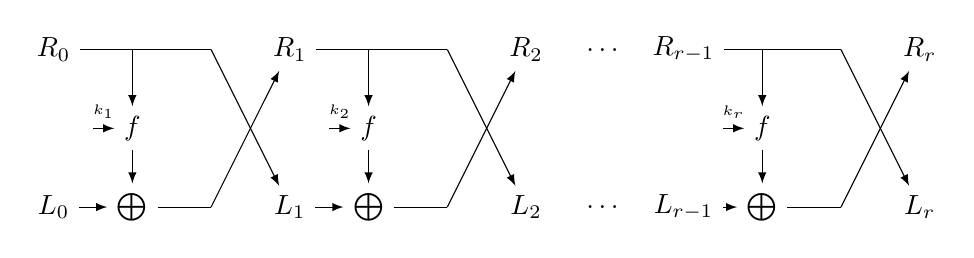
\begin{tikzpicture}[node distance=2cm,auto,>=latex]
  \node (R0) at (0,0)  {$R_0$};
  \node (L0) at (0,-2)  {$L_0$};
  \node (F0) at (1,-1)  {$f$};
  \node (xor0) at (1,-2)  {$\bigoplus$};
  \node (R1) at (3,0)  {$R_1$};
  \node (L1) at (3,-2)  {$L_1$};
  \node (F1) at (4,-1) {$f$};
  \node (xor1) at (4,-2)  {$\bigoplus$};
  \node (R2) at (6,0)  {$R_2$};
  \node (L2) at (6,-2) {$L_2$};
  \node at (7,0) {\dots};
  \node at (7,-2) {\dots};
  \node (Rr1) at (8,0) {$R_{r-1}$};
  \node (Lr1) at (8,-2)  {$L_{r-1}$};
  \node (Fr) at (9,-1) {$f$};
  \node (xorr) at (9,-2)  {$\bigoplus$};
  \node (Rr) at (11,0) {$R_{r}$};
  \node (Lr) at (11,-2)  {$L_{r}$};

  \draw[-] (R0) -> (2,0);
  \draw[->] (1,0) -> (F0);
  \draw[->] (L0) -> (xor0);
  \draw[->] (0.5,-1) -> node[above]{\tiny{$k_1$}} (F0);
  \draw[->] (F0) -> (xor0);
  \draw[-] (xor0) -> (2,-2);
  \draw[->] (2,0) -> (L1);
  \draw[->] (2,-2) -> (R1);

  \draw[-] (R1) -> (5,0);
  \draw[->] (4,0) -> (F1);
  \draw[->] (L1) -> (xor1);
  \draw[->] (3.5,-1) -> node[above]{\tiny{$k_2$}} (F1);
  \draw[->] (F1) -> (xor1);
  \draw[-] (xor1) -> (5,-2);
  \draw[->] (5,0) -> (L2);
  \draw[->] (5,-2) -> (R2);

  \draw[-] (Rr1) -> (10,0);
  \draw[->] (9,0) -> (Fr);
  \draw[->] (Lr1) -> (xorr);
  \draw[->] (8.5,-1) -> node[above]{\tiny{$k_r$}} (Fr);
  \draw[->] (Fr) -> (xorr);
  \draw[-] (xorr) -> (10,-2);
  \draw[->] (10,0) -> (Lr);
  \draw[->] (10,-2) -> (Rr);
\end{tikzpicture}
\end{center}

Dada a saída $\langle L_i, R_i \rangle$ da $i$-ésima rodada de uma rede de Feistel, podemos recuperar o valor de $\langle L_{i-1}, R_{i-1} \rangle$ primeiro fazendo $R_{i-1} := L_i$ e em seguinda calculando:
\begin{displaymath}
  L_{i-1} := R_i \xor f_i(R_{i-1})
\end{displaymath}

Esse procedimento pode ser repetido para todas as rodadas da rede para inverter a função.

O DES é uma rede de Feistel com 16 rodadas.
Ela recebe uma chave de 64 e prontamente descarta 8, portanto, e criptografa blocos de 64 bits, ou seja, $DES: \{0,1\}^{56} \times \{0,1\}^{64} \to \{0,1\}^{64}$.
A chave de 56 passa por um processo chamado {\em key schedule} que produz 16 subchaves de 48 bits.
As funções em cada rodada do DES são identicas, recebem uma subchave de 48 bits e um bloco de 32 bits (metade do bloco total) e produz um bloco de 32 bits $f: \{0,1\}^{48} \times \{0,1\}^{32} \to \{0,1\}^{32}$.
Resta, portanto, apresentar a função $f$ (Figura \ref{fig:feistel-function}):
\begin{enumerate}
\item o bloco é expandido para uma sequência de 48 bits,
\item aplica-se o XOR do bloco expandido com a subchave,
\item o resultado é dividido em 8 pedaços de 6 bits cada,
\item cada pedaço desses passa por um SBox diferente que substitui os 6 bits por 4 bits (fase de confusão),
\item o resultado é reduzido para uma sequência de 32 bits e, por fim,
\item os bits são misturados (fase de difusão).
\end{enumerate}

\begin{figure}[!htp]
  \centering
  \includegraphics[width=.4\textwidth]{imagens/feistel-function.png}
  \caption{Função de Fiestel do DES}
  \label{fig:feistel-function}
\end{figure}


A adoção do padrão DES foi cheia de controvérsias.
Não foi esclarecido o motivo do descarte do 8 bits da chave.
Uma chave de 56 bits é hoje considerada insegura contra um ataque de força bruta e estava no limite da segurança nos anos 70.
Um artigo de 1993 propõe um projeto de hardware que, em teoria, seria capaz de aplicar um ataque força-bruta em uma chave de 56 bits em um dia e meio \cite{}.
Em 1998 a {\em Eletronic Frontier Foundation} (EFF) construiu uma máquina que foi capaz de quebrar a cifra em 56 horas (cerca de dois dias e meio).
A máquina chamada de {\em Deep Crack} custou pouco menos de 250 mil dólares.
Em 2006 pesquisadores alemães desenvolveram um hardware de baixo custo -- cerca de dez mil dólares -- capaz de efetuar um ataque de força-bruta ao DES em menos de uma semana.
Desconfia-se que nos anos 80 apenas governos de grandes potências mundiais tinham recursos necessários para construir máquinas com tal capacidade.
Hoje em dia o algoritmo DES é considerado totalmente inseguro.

% No livro do Paar tem uma definição formal de ataque força bruta e uma análise da probabilidade de coincidência de chaves

Além do pequeno tamanho da chave, e mais suspeito, os S-Boxes foram alterados pela NSA sem grandes explicações antes do algoritmos ser adotado como padrão.
Anos mais tarde pesquisadores apresentaram uma técnica chamada criptoanálise diferencial.
Diversas cifras se tornaram inseguras com o anúncio desta técnica, mas supreendentemente o DES não.
Desconfia-se que os pesquisadores da NSA conheciam a técnica e alteraram a cifra de forma que ela se torna-se segura contra este tipo de ataque.

\subsection{Advanced Encryption Standard (AES)}
\label{sec:aes}

As desconfianças em torno do DES e o ataque força bruta iminete contra sua chave levaram o orgão estadunidense responsável pela estabelecimento de padrões internacionais (NIST) a propor um concurso acadêmico em 1997 para elaboração de um novo padrão.
Cada concorrente, além de propor o algoritmo tinha a tarefa de encontrar vulnerabilidades nos demais algoritmos propostos.
Cinco finalistas foram considerados adequados e em abril de 2000 o algoritmos {\em Rijndael} foi anunciado como vencedor e passou a ser chamado de AES.

O AES criptografa blocos de 128 bits possui três versões: uma com chaves de 128 bits e 10 rodadas, uma com chaves de 196 bits e 12 rodadas e uma com chaves de 256 bits e 14 rodadas.
Diferente do DES, o AES não usa uma rede de Feistel, mas uma técnica que chama-se {\em rede de substituição e permutação}.

O bloco no AES é dividido em 8 sequência de 16 bits que é tratada com um quadrado de 4 por 4 chamado de {\em estado}.
Em cada rodada o algoritmo repete os seguintes passos (Figura \ref{fig:aes}).

\begin{enumerate}
\item {\em AddRoundKey:} O {\em key schedule} do AES produz uma subchave de 128 bits para cada rodada e aplicamos o XOR dessa subchave com o estado.
\item {\em SubBytes:} Cada byte do estado é substituído por um novo byte definido por um SBox único que é bijetor (fase de confusão).
\item {\em ShiftRow:} Rotacionamos a segunda linha do estado em uma posição, a terceira em duas posições e a quarta e três posições para a direita.
\item {\em MixColumns:} As quatro linhas do estado são interpretados com um vetor que é multiplicado por uma matriz específica e fixa. Essa transformação é de tal forma que garante que cada byte de entrada influencie quatro bytes de saída (fase de difusão). 
\end{enumerate}

\begin{figure}[!htp]
  \centering
  \begin{minipage}{.45\textwidth}
    \centering
    \includegraphics[width=\textwidth]{imagens/AddRoundKey.png}  
  \end{minipage}
 \begin{minipage}{.45\textwidth}
    \centering
    \includegraphics[width=\textwidth]{imagens/SubBytes.png}
  \end{minipage}
  \begin{minipage}{.45\textwidth}
    \centering
    \includegraphics[width=\textwidth]{imagens/ShiftRows.png}  
  \end{minipage}
 \begin{minipage}{.45\textwidth}
    \centering
    \includegraphics[width=\textwidth]{imagens/MixColumns.png}
  \end{minipage}
  \caption{Etapas do AES}
  \label{fig:aes}
\end{figure}

Na última rodada a fase {\em MixColumn} é substituída pela {\em AddRoundKey}.
O AES é construído cuidadosamente de forma ser efecientemente inversível na presença da chave.
Até a escrita destas notas não se conhece um ataque contra o AES mais eficiente do que o ataque força bruta.




\section{Exercícios}
\label{sec:exercicios}

\begin{exercicio}
  Considere a definição de segurança contra CPA em que consideramos qualquer adversário $\mathcal{A}$ -- não apenas os eficientes -- e exigimos que $Pr[PrivK^{cpa}_{\Pi,\mathcal{A}}(n) = 1] = \frac{1}{2}$.
  Mostre que é impossível construir um sistema que satisfaça essa definição de segurança.
\end{exercicio}

\begin{exercicio}
Mostre que a operação $R_i \xor f_i(R_{i-1})$ na rede de Feistel de fato recupera o valor de $L_{i-1}$.
\end{exercicio}

\begin{exercicio}
  Mostre que os modos CBC e Ctr são corretos, ou seja, que em ambos os casos $D(k, E(k,m)) = m$;
\end{exercicio}

\begin{exercicio}
  Suponha que $f$ seja uma função pseudo-aleatória com chave e blocos ambos de 128 bits e considere o seguinte sistema:
  \begin{enumerate}
  \item Seleciona aleatoriamente duas sequência de 128 bits, a chave $k$ e o vetor inicial $IV$
  \item Divide a mensagem $m$ em blocos de 128 bits: $m_0, m_1, \dots, m_{n-1}$ (podemos supor que $|m|$ é múltiplo de 128).
  \item A cifra $c = c_0 || c_1 || \dots || c_{n-1}$ é tal que $c_i = m_i \oplus f_k(IV)$ para $i = 0, ..., n-1$
  \item Para descriptografar fazemos $c_i \oplus f_k(IV)$ para $i = 0, \dots, n-1$.
  \end{enumerate}
  Esse sistema é seguro? Por que?
\end{exercicio}

\begin{exercicio}
Suponha que um bit em uma cifra tenha sido alterado por um erro.
Qual o efeito disso na mensagem descriptografada caso a cifra tenha sido produzida usando o modo Ctr? E no caso de ter sido produzida usando o modo CBC?  
\end{exercicio}



